\part{Estructura cristalina}

\chapter{Redes de Bravais}
Una red se denota \emph{de Bravais} si se ve igual desde todos los
puntos. Una red hexagonal no lo es, por ejemplo, ya que en ciertos
puntos la red se ve invertida verticalmente respecto a otros (fig. \ref{fig:hexa}).
\begin{figure}
  \centering
  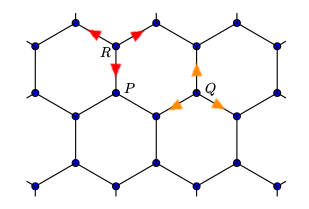
\includegraphics[width=0.5\textwidth]{figures/hexa.png}
  \caption{Las redes hexagonales no son redes de Bravais, ya que en
    distintos puntos (R,Q) se ve un entorno distinto (en este caso,
    invertido verticalmente).}
  \label{fig:hexa}
\end{figure}

De manera rigurosa, una red de Bravais es el conjunto de todos los
infinitos puntos con vectores de posición
\begin{equation}
  \mathbf{R} = n_1 \mathbf{a}_1 + n_2 \mathbf{a}_2  + n_3 \mathbf{a}_3
\end{equation}
con $\mathbf{a}_i$ vectores no coplanares, cuya elección no es
única. Se definen algunos conceptos relacionados:
\begin{description}
\item[Vectores (base) primitivos] El triplete $\mathbf{a}_i$.
\item [Celda] Volumen del espacio que al trasladarlo por toda la red
  llena el espacio sin solaparse ni dejar agujeros. Un ejemplo es el
  paralelepípedo definido por
  $\mathbf{a}_1,\mathbf{a}_2,\mathbf{a}_3$, de volumen
  $\Omega = \mathbf{a}_1 \cdot (\mathbf{a}_2 \times \mathbf{a}_3)$. 
  \begin{description}
  \item[Celda primitiva] Si una celda es primitiva, sólo contiene un
    punto de la red\footnote{Recordar que hay que pintar los puntos
      ``gordos'': en un cuadrado con un punto en cada arista, por
      ejemplo, cada punto sólo vale $1/4$ (si fueran círculos, sólo
      habría $1/4$ dentro del área del cuadrado) y por tanto hay un
      solo punto.}. 

    Un tipo especial de celda primitiva es la \emph{celda de
      Wigner-Seitz}. Dado un punto (que contiene la celda), es el
    espacio geométrico de los puntos que están más cerca de dicho
    punto que de cualquier otro. Si el sistema no es una red de
    Bravais, el concepto homólogo es un diagrama de Voronoi.
    
    Las distintas celdas primitivas siempre tienen el mismo volumen.
  \item[Celda convencional] Celda no primitiva.  Las celdas
    convencionales siempre tienen más puntos y más volumen que las
    primitivas.
  \end{description}
  Pueden verse ejemplos de las tres celdas en la figura \ref{fig:celdas}.
\item[Base (atómica)] Motivo (por ejemplo, un conjunto de átomos) que
  se asocia a \emph{todos} los puntos de la red. Notar que la red en
  sí no tiene ningún elemento, es sólo una descripción geométrica
  hasta que se ``rellena'' con una base.
\item[Estructura cristalina (Cristal)] Unión de una base y una red.
\end{description}
\begin{figure}
  \centering
  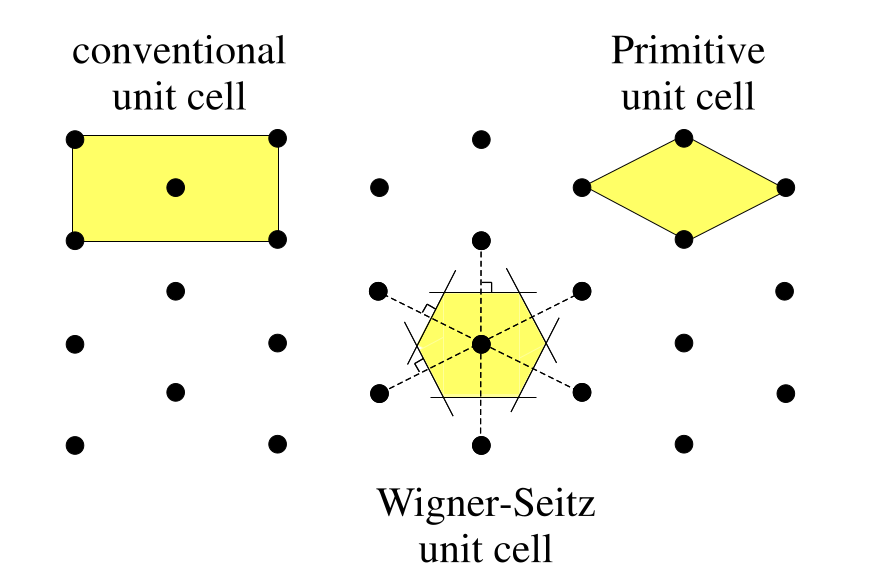
\includegraphics[width=0.7\textwidth]{figures/celdas.png}
  \caption{Distintos tipos de celdas en una red triangular. Excepto la
    convencional (que contiene dos), las otras dos contienen un único
    punto.}
  \label{fig:celdas}
\end{figure}

\section{Redes cúbicas}
Sólo existen tres redes cúbicas de Bravais (fig. \ref{fig:cubes}).

\subsection{Simple Cubic} 
La más simple es la red \emph{Simple Cubic}, SC. Los vectores
  base más obvios son tres aristas, con origen en alguna esquina. El
  paralelepípedo que definen es una celda primitiva, con $\Omega = a^3$.

  Su número de vecinos (o de \emph{coordinación}) es 6.
\subsection{Body-Centered Cubic} 
La red \emph{Body-Centered Cubic} (BCC o Cubic-I) es similar a la SC pero
  con un punto extra dentro de la celda anterior. Ahora la celda no es
  convencional (tiene dos puntos).

  Un cristal BCC puede expresarse como una SC con una base de dos
  átomos\footnote{Recordar que una base de átomos se repite tantas
    veces como puntos de la red (una vez en cada origen de
    coordenadas). Esto implica que para un cubo (8 nodos, 8 orígenes,
    8 aristas) la base se repite 8 veces. En las imágenes se muestra
    sólo el átomo de dentro de la celda, pero una representación de la
    BCC como SC con base de dos átomos debería mostrar las 8 aristas
    en azul y 8 átomos en morado; el de dentro del cubo
    (correspondiente al nodo inferior izquierdo, en la cara que no
    está oculta) y los 7 restantes en las posiciones
    $x _{\text{arista}} + (0.5,0.5,0.5)$.}:
\begin{equation}
  \text{BCC} = \text{SC} + \text{Base},\ \ \ \text{Base} =
  \begin{cases}
    (0,0,0)_{\text{at. tipo 1}} \\
    (\frac{1}{2},\frac{1}{2},\frac{1}{2})_{\text{at. tipo 2}}
  \end{cases}
\end{equation}
Hay elecciones de ejes más interesantes si no se quiere recurrir a
descomponerla en una base. En la figura \ref{fig:cubeaxis} se muestran
dos conjuntos:
\begin{itemize}
\item Los ejes negros ($\mathbf{a}_i$) corresponden a unir la
arista con los puntos centrales de las celdas adyacentes.
\begin{equation}
    \{\mathbf{a}_i\}  =
    \begin{cases}
      \mathbf{a}_1 =  \frac{a}{2} (-\hat{\mathbf{x}} + \hat{\mathbf{y}} +
      \hat{ \mathbf{z}} ) \\
      \mathbf{a}_2 =  \frac{a}{2} (\hat{\mathbf{x}} + -\hat{\mathbf{y}} +
      \hat{ \mathbf{z}} ) \\
      \mathbf{a}_3 = \frac{a}{2} (\hat{\mathbf{x}} + \hat{\mathbf{y}} +
      -\hat{ \mathbf{z}} )
    \end{cases}
\end{equation}
\item Los ejes rojos ($\mathbf{b}_i$) corresponden a la unión de la arista con
  las dos aristas adyacentes de la base y con el punto del centro de
  la celda.

\begin{equation}
    \{\mathbf{b}_{i}\} =
    \begin{cases}
      \mathbf{b}_1 = a \hat{\mathbf{x}} \\
      \mathbf{b}_2 = a \hat{\mathbf{y}} \\
      \mathbf{b}_3 = \frac{a}{2} (\hat{\mathbf{x}} + \hat{\mathbf{y}}
      + \hat{ \mathbf{z}} )
    \end{cases}
  \end{equation}
\end{itemize}
En ambos casos, las celdas primitivas correspondientes tienen
 $\Omega = a^3/2$.

Su número de coordinación es 8.
\begin{figure}
  \centering
  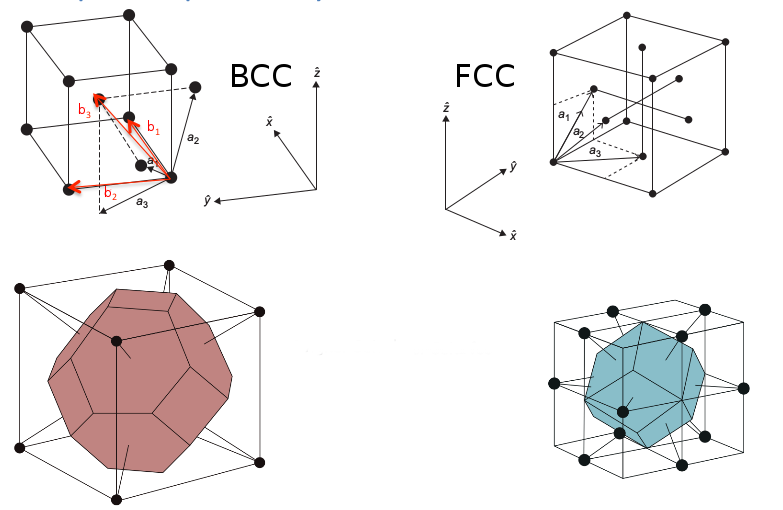
\includegraphics[width=\textwidth]{figures/cubeaxis.png}
  \caption{Ejes para redes FCC y BCC. Se muestran también sus celdas
    de Wigner-Seitz.}
  \label{fig:cubeaxis}
\end{figure}

\subsection{Face-Centered Cubic}
La red \emph{Face-Centered Cubic}, FCC o Cubic-F contiene un
  punto extra en cada cara del cubo. La celda cúbica contiene 4
  puntos. Si se expresa como una SC con una base, queda como
\begin{equation}
  \text{FCC} = \text{SC} + \text{Base},\ \ \ \text{Base} =
  \begin{cases}
    (0,0,0)_{\text{at. of kind 1}} \\
    (\frac{1}{2},\frac{1}{2},0)_{\text{at. of kind 2}} \\
    (\frac{1}{2},0,\frac{1}{2})_{\text{at. of kind 2}} \\
    (0,\frac{1}{2},\frac{1}{2})_{\text{at. of kind 2}} \\
  \end{cases}
\end{equation}
con un átomo por origen de un tipo y tres extra en los centros de las
caras del triedro definido por los ejes. 

Si se quieren unos ejes que no obliguen a esta descomposición, se
puede recurrir a los de la figura \ref{fig:cubeaxis}:
\begin{equation}
  \{\mathbf{a}_i\} =
  \begin{cases}
     \mathbf{a}_1 = \frac{a}{2} ( \hat{ \mathbf{y}} + \hat{ \mathbf{z}} )  \\
      \mathbf{a}_2 = \frac{a}{2} (\hat {\mathbf{x} }+ \hat {\mathbf{z} })   \\
      \mathbf{a}_3 = \frac{a}{2} (\hat {\mathbf{x}} + \hat {\mathbf{y} }) 
  \end{cases}
\end{equation}
Con estos ejes $\{\mathbf{a}_i\}$, la celda tiene $\Omega = a^3/4$.

Su número de coordinación es 12.
\begin{figure}
  \centering
  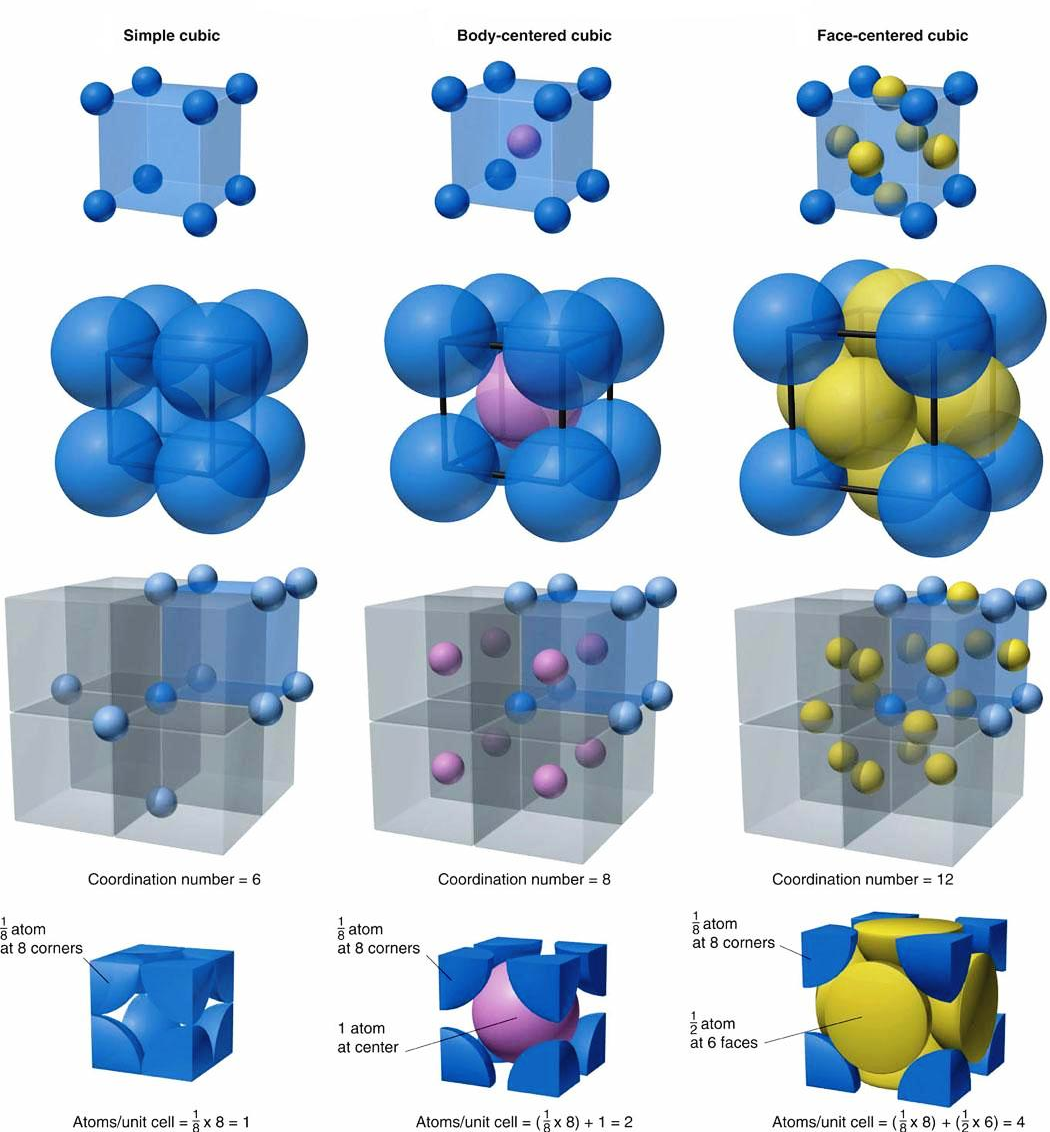
\includegraphics[width=\textwidth]{figures/cubes.png}
  \caption{Redes de Bravais cúbicas.}
  \label{fig:cubes}
\end{figure}


\subsection{Clasificación de estructuras}
Podemos plantearnos conjuntos de operaciones que, tras aplicarlas en
redes, dejen estas en su estado original:
\begin{enumerate}
\item Traslaciones sobre los vectores de la red.
\item Operaciones que dejan fijo un punto de la red.
\item Combinaciones de los anteriores.
\end{enumerate}

Estas operaciones se agrupan en los llamados \emph{grupos
  puntuales} y \emph{grupos espaciales}, representados en la figura \ref{fig:bravaisgroups}.
\begin{itemize}
\item Los grupos puntuales son los que consideran sólo operaciones que dejan
fijo un punto de la red. Existen (para redes de Bravais) 7 distintos.
\item Los grupos espaciales son más laxos y permiten también las
traslaciones. En redes de Bravais, existen 14.
\end{itemize}


\begin{figure}
  \centering
  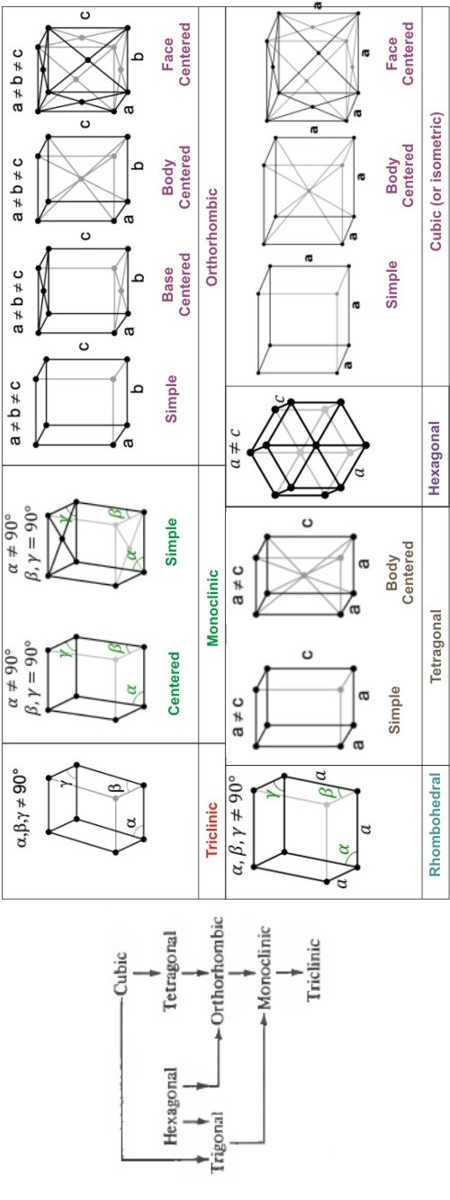
\includegraphics[width=0.5\textwidth]{figures/bravaisgroups.png}
  \caption{El grupo puntual más simétrico es el cúbico (las flechas indican pérdida de simetría conforme se realizan deformaciones). Al incluir traslaciones los 7 grupos puntuales se expanden en 14 espaciales.}
  \label{fig:bravaisgroups}
\end{figure}

Si no nos ceñimos a redes de Bravais, se obtienen 32 grupos puntuales
de estructuras cristalinas y más de 200 grupos espaciales.

\section{La red recíproca}
Hasta ahora siempre hemos trabajado con la red directa (en el espacio
real). Una representación alternativa (similar a la representación en
espacio de Fourier) es la red recíproca. Se define como el conjunto de
los $\mathbf{k}$ que tienen la misma periodicidad que la red.
\begin{definition}[Red recíproca]
  Sea una red de Bravais $\mathbf{R}$, y una onda plana
  $e ^{i\mathbf{k}\mathbf{r}}$. Se conoce como red recíproca a los
  vectores $\mathbf{k}$, que cumplen
  \begin{equation}
    e ^{i\mathbf{k}(\mathbf{r}+\mathbf{R})} = e ^{i\mathbf{k}\mathbf{r}} \rightarrow e ^{i\mathbf{k}\mathbf{R}}=1, \ \forall\mathbf{R}
  \end{equation}
  A estos vectores se les denota $\mathbf{G}$.
\end{definition}
La celda de Wigner-Seitz de la red recíproca se conoce como
\emph{primera zona de Brillouin}.

\subsection{Vectores primitivos de la red recíproca}
Sea $\Omega = \mathbf{a}_1 \cdot (\mathbf{a}_2 \times \mathbf{a}_3)$,
se tiene que $\mathbf{G} = m_1 \mathbf{b}_1 + m_2 \mathbf{b}_2 + m_3
\mathbf{b}_3$ donde las $\mathbf{b}_i$ valen
\begin{equation}
  \begin{cases}
    \mathbf{b}_1 &= 2\pi \frac{\mathbf{a}_2 \times \mathbf{a}_3}{\Omega} \\
    \mathbf{b}_2 &= 2\pi \frac{\mathbf{a}_3 \times \mathbf{a}_1}{\Omega} \\
    \mathbf{b}_3 &= 2\pi \frac{\mathbf{a}_1 \times \mathbf{a}_2}{\Omega} \\
  \end{cases}
\end{equation}
Además $\mathbf{b}_i \mathbf{a}_j = 2\pi \delta _i^j$ y 
\begin{equation}
  \Omega_k = \mathbf{b}_1 \cdot (\mathbf{b}_2 \times \mathbf{b}_3) = \frac{(2\pi)^3}{\Omega}
\end{equation}


\section{Funciones periódicas}
\label{sec:fper}
El potencial de la red es periódico
($f(\mathbf{r}) = f (\mathbf{r}+\mathbf{R})$). Puedo expandirlo por
tanto en serie de funciones periódicas. Utilizo para ello las $\mathbf{G}$:
\begin{equation}
  f(\mathbf{r}) = \sum_\mathbf{G} f_\mathbf{G} e ^{i\mathbf{G}\mathbf{r}}
\end{equation}
Para obtener los coeficientes $f _{\mathbf{G}}$ actúo como en una
serie de Fourier normal. Comienzo por multiplicar por $e ^{-i\mathbf{G'}\mathbf{r}}$:
\begin{equation}
  f(\mathbf{r})e ^{-i\mathbf{G'}\mathbf{r}} = \sum_\mathbf{G} f_\mathbf{G} e ^{i\mathbf{r}(\mathbf{G}-\mathbf{G'})}
\label{eq:temporal4565}
\end{equation}
Integro en una celda primitiva. Para ello, necesito el siguiente lema:
\begin{lemma}
  Sea $\Omega$ la región de una celda primitiva.
  \begin{equation}
    \label{eq:lemmaomega}
    \myiiint_\Omega \text{d}\mathbf{r} e ^{i\mathbf{G}\mathbf{r}}=\Omega\  \delta_{\mathbf{G},\mathbf{0}}
  \end{equation}
  \begin{boldproof}
    Para $\mathbf{G} = 0$ es trivial, ya que se obtiene $\iiint_\Omega \text{d}\mathbf{r} $ que no es más que $ \Omega$.

    Para $\mathbf{G}\neq0$, escribo el vector como
    $\mathbf{G} = h \mathbf{b}_1 + k \mathbf{b}_2 + l \mathbf{b}_3$,
    con $h,k,l \in \mathbb{Z}$. Expreso $\mathbf{r}$ como
    $x \mathbf{a}_1 + y \mathbf{a}_2 + z \mathbf{a}_3$, y al limitarme
    a una celda unidad $0 \leq x,y,z \leq 1$. 

    El producto $\mathbf{G}\mathbf{r}$ (recordar que $\mathbf{a}_i\mathbf{b}_j = 2\pi \delta_{i,j}$) es $2\pi(hx+ky+lz)$, introduciendo eso en la integral:
    \begin{equation}
      \myiiint_\Omega \text{d}\mathbf{r} e ^{i\mathbf{G}\mathbf{r}} =
      \underbrace{ \int_0^1 \text{d}\mathbf{x} e ^{i2\pi hx}}_{\mathclap{=0 (\text{full cicle})}}  
       \underbrace{ \int_0^1 \text{d}\mathbf{y} e ^{i2\pi ky}}  _{\mathclap{=0 (\text{full cicle})}}  
  \underbrace{      \int_0^1 \text{d}\mathbf{z} e ^{i2\pi lz}}_{\mathclap{=0 (\text{full cicle})}}   = 0 \cdot 0 \cdot 0 = 0  
    \end{equation}
  \end{boldproof}
\end{lemma}
Conocido este lema, puedo integrar la ecuación \ref{eq:temporal4565}:
\begin{equation}
\begin{split}
  \myiiint_\Omega \text{d}\mathbf{r} f (\mathbf{r})e ^{i\mathbf{G'}\mathbf{r}} &= \sum_\mathbf{G} f_\mathbf{G} \myiiint_\Omega \text{d}\mathbf{r} \ e ^{-i(\mathbf{G}-\mathbf{G'})\mathbf{r}} \\
  &= \sum_\mathbf{G} \Omega \delta_{\mathbf{G},\mathbf{G'}} = \Omega f_\mathbf{G'}
\end{split}
\end{equation}
Resultando
\begin{equation}
  f_\mathbf{G'} = \frac{1}{\Omega} \myiiint _\Omega \text{d}\mathbf{r} f (\mathbf{r})e ^{i\mathbf{G'}\mathbf{r}}
\end{equation}

\section{Planos cristalinos}
Se denota \emph{familia de planos cristalinos} a un conjunto de planos
equiespaciados que contienen a todos los puntos de la red. En una red
cúbica, por ejemplo, la familia que contiene a una cara del cubo de la
celda convencional y todos los paralelos a distancia
$\Omega^{1/3}$. Se relacionan con la red recíproca mediante el siguiente teorema:
\begin{theorem}
\label{thm:reciprocidad}
  Sea una familia de planos separados por una distancia $d$. Existen
  vectores en la red recíproca que son normales a la familia, el más
  corto de ellos con módulo $2\pi /d$.

  De manera recíproca, para cualquier vector $\mathbf{G}$ de la red
  recíproca existe una familia de planos perpendiculares a éste con
  separación $d$, siendo $2\pi /d$ el módulo del vector más corto
  paralelo a $\mathbf{G}$.
\end{theorem}

\section{Índices de Miller}
El teorema \ref{thm:reciprocidad} nos muestra una posible notación
para identificar familias de planos en función de sus vectores en la
red recíproca. Sea
$\mathbf{G} = h \mathbf{b}_1 + k \mathbf{b}_2 + l\mathbf{b}_3$, al set
$(h k l)$ se le denota \emph{índices de Miller}.  Dependen de la celda
usada, no son únicos para cada familia de planos. La notación tiene
ciertas peculiaridades:
\begin{itemize}
\item Los números negativos se escriben con una barra encima.
\item No se utilizan comas para separar los índices
\item En simetría hexagonal, se suele usar un cuarto índice
  $i=-(h+k)$, quedando los índices $(h \ k\  i\  l)$.
\end{itemize}
Con esta notación, algo como $(1,-3,2)$ se escribiría $(1 \ \bar 3 \ 2)$.

Hasta ahora sólo se han indexado planos. Para indexar direcciones en
el espacio se utilizan corchetes, de tal forma que la dirección del vector paralelo a
$\mathbf{R} = h \mathbf{a}_1 + k\mathbf{a}_2 + l \mathbf{a}_3$ más corto\footnote{Con más corto nos referimos a transformar $[0\ 0\ 3]$, por ejemplo, en $[0\ 0\ 1]$. Hay que recordar que $h,k,l$ son enteros, siendo el valor más pequeño posible $1$. Por ejemplo, $[\frac{1}{2}\ \frac{1}{2}\ \frac{1}{2}]$ no son índices válidos.} queda
como $[h\ k\ l]$. 

Los planos equivalentes por simetría se denotan $\langle h\ k\ l\rangle$. Por ejemplo,
\begin{equation*}
  \langle 0 \ 0 \ 1\rangle = \{ [1\  0\  0], [0\  1\  0], [0\  0\  1], [\bar 1\  0\  0], [0\  \bar 1\  0], [0\  0\  \bar 1]\}
\end{equation*}

$[h\ k\ l]$ en general no es perpendicular a $(h \ k\ l)$, excepto en el sistema cúbico.

\paragraph{Ejemplo de cálculo}
Tenemos un plano en el espacio discreto que corta los ejes
$\mathbf{a}_i$ en $(2,2,3)$. Para calcular sus índices de Miller,
calculamos los inversos de los puntos de corte:
\begin{equation*}
 \left(\frac{1}{2},\frac{1}{2},\frac{1}{3}\right)
\end{equation*}
A continuación, dividimos por el GCD:
\begin{equation*}
 (3,3,2)
\end{equation*}
Los índices de Miller son $(3\ 3\ 2)$.

Si no hay corte con algún eje, se supone que el corte es en
$\sim \infty$ y se aproxima $\frac{1}{\sim \infty} \sim 0$ cuando se
invierte.

\chapter{Determinación de estructuras}

Para poder resolver las estructuras internas de los cristales, necesitamos
sondas con $\lambda \sim \AA$.
\begin{description}
\item[Fotones] Se utilizan rayos X. Tienen que tener una energía de
  aproximadamente 10 keV, y tienen la ventaja de ser baratos y no desviarse por
  interacciones con la muestra.
\item[Electrones] Es necesario que posean unos 100 eV. Al estar cargados,
  interaccionan fuertemente con las nubes electrónicas y tienen poco poder de
  penetración.
\item[Neutrones] La resolución que aportan es brutal, pero son muy caros.
  Además, es necesario reducir su energía a decenas de meV (a esa energía, se
  les denota \emph{neutrones térmicos}, por ser su energía aproximadamente
  $\kb T$.)

  Como no tienen carga, su interacción con las nubes electrónicas es
  despreciable, lo que determina su gran resolución. No obstante, como poseen
  spin hay una débil interacción con los electrones que nos permite estudiar
  interacciones magnéticas.

  El flujo de neutrones de un reactor nuclear dedicado es brutal, lo que me
  permite realizar en 10 minutos lo que necesitaría radiación de rayos X durante
  un mes.
\end{description}

\section{Teoría mecanocuántica del scattering}
Es razonable suponer que a la salida del cristal tendré algo parecido a
\begin{equation}
  \underbrace{\psi(\mathbf{r})}_{\mathclap{\text{out}}} = \underbrace{e ^{i \mathbf{k}\mathbf{r}}}_{\text{no scattered}} + \underbrace{f\cdot \frac{e ^{i \mathbf{k}\mathbf{r}}}{r}}_{\text{scattered}}
\end{equation}
y que la sección eficaz será algo similar a
\begin{equation}
  \frac{\text{d}\sigma}{\text{d}\Omega} \sim \vert f \vert ^2
\end{equation}

Para calcularlo de manera rigurosa, recurrimos a la ecuación de Lipman-Swinger,
que es prácticamente la ecuación de Schrodinger en forma integral:
\begin{equation}
  \psi _{\mathbf{k'} } (\mathbf{r}) = e ^{i\mathbf{k}\mathbf{r}} - \frac{1}{4\pi} \int \text{d}\mathbf{r'}  \frac{e ^{i \mathbf{k}\vert \mathbf{r}-\mathbf{r}' \vert}}{\vert \mathbf{r}-\mathbf{r}' \vert} U(\mathbf{r}') \psi _{\mathbf{k}}(\mathbf{r'}) 
\end{equation}
donde $U(\mathbf{r}') = \frac{2m}{\hbar^2}V(\mathbf{r}')$.

La ecuación es muy difícil de resolver, por lo que una aproximación a distancias
de detección grandes resulta especialmente útil. Para $r \gg r'$ se obtiene:
\begin{equation}
  \psi _{\mathbf{k'}} (\mathbf{r}) = e ^{i\mathbf{k}\mathbf{r}} + f(\theta,\psi) \frac{e ^{i\mathbf{k}\mathbf{r}}}{r}
\end{equation}
que es similar a nuestra hipótesis de partida, siendo la amplitud del
scattering $f$, llamada \emph{función de Born}. Hagamos una expansión en series
de Born:
\begin{equation}
\label{eq:borneq}
  f _{\text{Born}} = \frac{-1}{4\pi} \langle \mathbf{k}' \vert U \vert \mathbf{k} \rangle
\end{equation}
que no es más que la regla de oro de Fermi ( $f _{\text{Born}} = \frac{-1}{4\pi}
\langle \boldsymbol{\phi}' \vert U \vert \boldsymbol{\phi} \rangle$ ).

\section{Formulaciones clásicas}
Las principales son las de Bragg y Laue. En el fondo, una es la transformada de
Fourier de la otra.

\subsection{Bragg}
Partimos de una serie de suposiciones:
\begin{itemize}
\item Un cristal es un conjunto de planos equiespaciados.
\item La reflexión de la sonda utilizada en dichos planos es especular.
\item Suponemos que hay interferencia constructiva de los rayos en diferentes
  planos.
\end{itemize}
Con estas condiciones, y un poco de geometría (ver desarrollo en los apuntes de
óptica, por ejemplo), se llega a la siguiente expresión:
\begin{equation}
  \boxed{ 2d\sin(\theta) = n\lambda
 }\end{equation}

\subsection{Laue}
En este caso, prescindo de la hipótesis de los planos del cristal. Veo el
cristal como una serie de centros dispersores, que al ser incididos radian en
todas las direcciones del espacio.

Imaginemos dos centros dispersores, como los de la figura \ref{fig:laue_geom}.
Definimos los vectores de onda $ \mathbf{k}=\frac{2\pi}{\lambda} \hat n$ y $
\mathbf{k'}=\frac{2\pi}{\lambda} \hat n'$. Sea una interacción elástica, lo que
implica que $k=k'$. Notar que esto no tiene por qué ser así, pero supóngase.

La diferencia de caminos es 
\begin{equation}
\begin{split}
  \Delta &= d \cos(\theta) + d \cos(\theta') \\
         &= \mathbf{d} (\hat n - \hat n ') = \\
         &= \frac{\lambda}{2\pi} \mathbf{d} (\mathbf{k}-\mathbf{k}')= \\
         &= m\lambda
\end{split}
\end{equation}
Por lo que obtenemos, simplificando $\lambda$ en los últimos pasos
\begin{equation}
  \mathbf{d}(\mathbf{k}-\mathbf{k}') = 2\pi m
  \label{eq:templab123}
\end{equation}
Recordamos que estamos en una red de Bravais, por lo que
$\mathbf{d}=\mathbf{R}$. Utilizando esto en la ec. \ref{eq:templab123} se llega
la condición de Laue:
\begin{equation}
\begin{split}
  \mathbf{R}(\mathbf{k}-\mathbf{k}') &= 2\pi m \\
  e ^{\mathbf{R}(\mathbf{k}-\mathbf{k}')} = e ^{2\pi m} &= 1, \ \ \forall m
\end{split}
\end{equation}
y por tanto

\begin{equation}
  \label{eq:lauecond}
\mathbf{k}-\mathbf{k'} = \mathbf{G}
\end{equation}

\begin{figure}
  \centering
  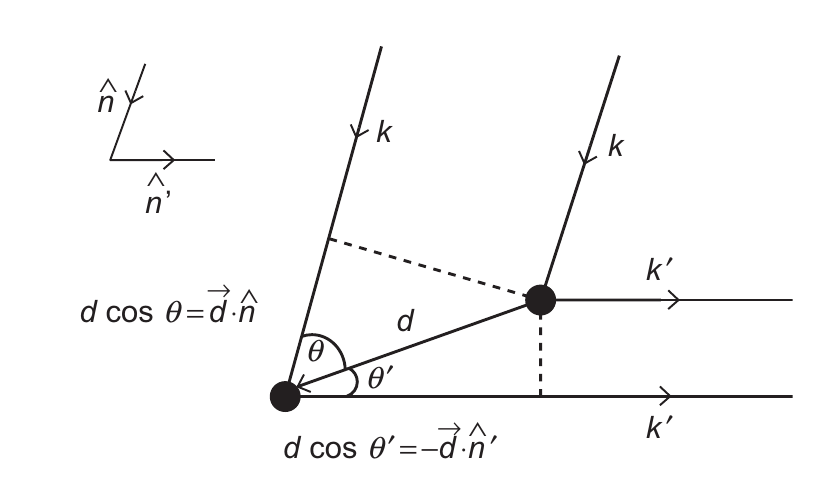
\includegraphics[width=\textwidth]{figures/laue_geom.png}
  \caption{Dos centros dispersores del modelo de Laue.}
  \label{fig:laue_geom}
\end{figure}

La condición de Laue (eq. \ref{eq:lauecond}) se puede escribir de manera
alternativa; como $\mathbf{k}'=\mathbf{k}-\mathbf{G}$, 
tenemos $k = k' = \vert \mathbf{k} - \mathbf{G}\vert $ 
y por tanto $k^2 = k^2 + G^2 - 2 \mathbf{k}\mathbf{G}$. 
De ahí despejamos $G^2 = 2\mathbf{k}\mathbf{G} =2\mathbf{k} \hat{\mathbf{G}} G$,
obteniendo
\begin{equation}
  \label{eq:lauealt}
  \mathbf{k}\hat { \mathbf{G} } = \frac{1}{2} G
\end{equation}
La nueva ecuación (eq. \ref{eq:lauealt}) me dice que si tengo 2 puntos de la red
recíproca, se cumple la situación geométrica de la figura \ref{fig:bragggeom}.
\begin{figure}
  \centering
  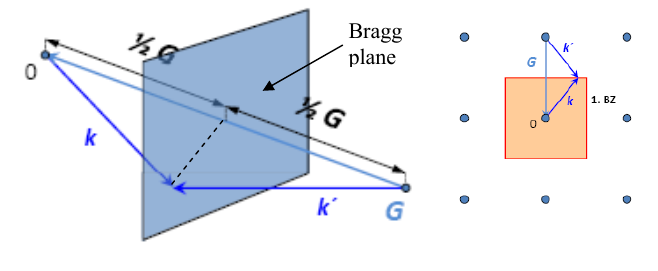
\includegraphics[width=\textwidth]{figures/bragggeom.png}
  \caption{La condición de Laue, en la forma de la ecuación
    \ref{eq:lauealt}, nos remite a los \emph{planos de Bragg},
    a los cuales $\mathbf{G}$ es perpendicular. Las zonas de Brillouin
    se pueden definir como regiones del espacio delimitadas
    por planos de Bragg, siendo la $i$-ésima zona de Brillouin aquella en
    que para llegar al punto de red es necesario cruzar, como mínimo,
    $i$ planos de Bragg.}
  \label{fig:bragggeom}
\end{figure}

La formulación de Laue incluye a la de Bragg; sólo hay que analizar con detenimiento una situación como la de la figura \ref{fig:lauebragg}, y utilizar lo que se sabe de la red recíproca.
Partamos de la eq. \ref{eq:lauealt} y utilicemos, viendo la figura
\ref{fig:lauebragg}, que $\frac{1}{2} G=k\sin(\theta)$.
\begin{equation}
  \frac{1}{2}G = k \sin \theta \ \rightarrow \ \underbrace{G}_{\mathclap{=mG_{min}}} = 2k \sin \theta 
\end{equation}
Conocemos que $G_{min}$ es, por el teorema de reciprocidad ya visto,
$\frac{2\pi}{d}$. Por tanto, al sustituir, obtenemos la condición de
Bragg ($m\lambda = 2d \sin \theta$).
\begin{figure}
  \centering
  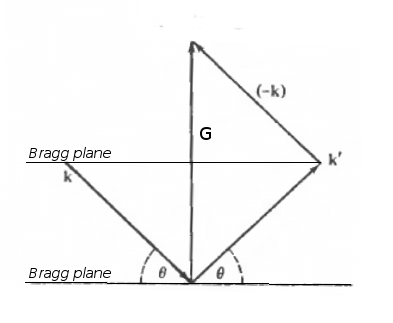
\includegraphics[width=0.5\textwidth]{figures/lauebragg.png}
  \caption{La formulación de Laue incluye a la de Bragg.}
  \label{fig:lauebragg}
\end{figure}


\subsubsection{Esfera de Ewald}
Imaginemos la \textbf{k} incidente. Sea el vector de módulo $k$ que, con la
dirección marcada por la geometría experimental (y por la incidencia de la sonda
en la muestra), acaba en un punto de la red. Girando ese vector por su punto de
aplicación, en los ángulos polares $\theta$ y $\phi$, se obtiene una esfera,
denotada \emph{esfera de Ewald}. Cualquier punto que caiga dentro verifica
automáticamente la condición de Laue ($\Delta \mathbf{k} = \mathbf{G}$), y por tanto en ellos hay difracción.

\begin{figure}[h]
  \centering
  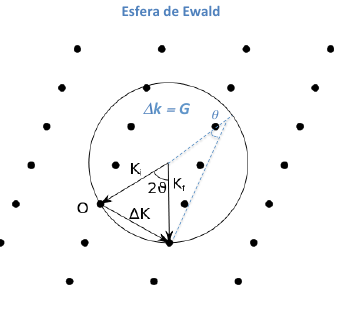
\includegraphics[width=0.6\textwidth]{figures/ewaldsphere.png}
  \caption{Construcción de una esfera de Ewald.}
\end{figure}


\subsection{Factor de estructura}
Vista la posibilidad de difracción, nos preguntamos cuál será la intensidad de
los picos. Recuperamos la ecuación de Born ya hallada en el análisis
mecanocuántico (eq. \ref{eq:borneq}) y tratamos de resolverla, ya que la
intensidad depende de ésta como $I \propto \vert f_{Born} \vert^2 $.
Resolver la integral nos da un parámetro denotado \emph{factor de
estructura}.
\begin{equation}
  \langle  \mathbf{k}' \vert V(\mathbf{r}) \vert \mathbf{k} \rangle \propto \myiiint \text{d}\mathbf{r} e ^{-i\mathbf{k'}\mathbf{r}} V(\mathbf{r})e ^{i\mathbf{k}\mathbf{r}} = \myiiint \text{d}\mathbf{r} e ^{-i \mathbf{r} (\mathbf{k'}-\mathbf{k})} V(\mathbf{r}) = \dots
\end{equation}
La normalización es indiferente, la absorbo en el prefactor junto a la resolución instrumental, etc.

Sea $\mathbf{r} = \mathbf{R}+\mathbf{x}$, con $\mathbf{x}$ limitado a la celda
unidad. Sumando sobre celdas,
\begin{equation}
\begin{split}
  \label{eq:samplitude}
  \dots &= \sum_{\text{cells}} \myiiint_{\text{cell}} \text{d}\mathbf{x} e ^{-i(\mathbf{R}+\mathbf{x})(\mathbf{k'}-\mathbf{k})} \underbrace{V(\mathbf{R}+\mathbf{x})}_{\mathclap{=V(\mathbf{x}) \text{(periodic)}}} =\\ &= \sum_{\text{cells}} e ^{-i (\mathbf{k'}-\mathbf{k})\mathbf{R}} \myiiint_{\text{cell}} \text{d}\mathbf{x} e ^{-i (\mathbf{k'}-\mathbf{k})\mathbf{x}} V(\mathbf{x}) = \dots
\end{split}
\end{equation}
Utilizando la igualdad $\sum_\mathbf{R}
e^{-i(\mathbf{k'}-\mathbf{k})\mathbf{R}}=N
{\delta(\mathbf{k'}-\mathbf{k},\mathbf{G})}$ (apéndice \ref{chap:latticesum}), llegamos a 
\begin{equation}
  \dots = N_{\text{cells}} \underbrace{\myiiint_{\text{cell}} \text{d}\mathbf{x} e ^{-i\mathbf{G}\mathbf{x}} V(\mathbf{x})
}_{\mathclap{F(\mathbf{G})\text{, structure factor}}}
\end{equation}
llegamos así a que $I \propto N^2 \vert F(\mathbf{G})\vert^2$. Con un cristal
grande ($N \gg$) se obtienen picos de más intensidad ($I \propto N^2$) y más
estrechos ($A \propto 1/N$). 

\subsection{Factor de forma}
\label{subsec:formfactor}

El potencial puede ser arbitrariamente complicado, así que se realiza la
aproximación
\begin{equation}
  V(\mathbf{x}) \sim \sum_j V_j(\mathbf{x}-\mathbf{x}_j)
\end{equation}
donde los $j$ son los elementos dispersores ($j \in (1,N_\text{atoms})$). Con
ello el factor de estructura se reduce a
\begin{equation}
\begin{split}
  F(\mathbf{G}) &= \myiiint_\text{cell} \text{d}\mathbf{x} e ^{-i\mathbf{G}\mathbf{x}}\sum_j V_j (\mathbf{x}-\mathbf{x}_j)  \stackrel{\mathbf{x}-\mathbf{x}_j=\boldsymbol{\rho}}{=} \\
                &= \sum_j \myiiint_\text{cell} \text{d}\boldsymbol{\rho} e ^{-\mathbf{G}(\boldsymbol{\rho}+\mathbf{x}_j)}V_j(\boldsymbol{\rho}) = \\
                &= \sum_j e ^{-i\mathbf{G}\mathbf{x_j}} \underbrace{\myiiint_\text{cell}\text{d}\boldsymbol{\rho}e ^{-i\mathbf{G}\boldsymbol{\rho}}V_j(\boldsymbol{\rho})}_{f_j (\text{atomic form factor})} = \\
&= \sum_j f_j e ^{-i\mathbf{G}\mathbf{x}_j}
\end{split}
\end{equation}
Si me han dado el valor de $f_j$ para cada átomo, el problema se reduce a sumar.

\subsubsection{Rayos X}
Veamos, por ejemplo, su valor para rayos X. Los centros dispersores son
electrones, así que $V_j(\boldsymbol{\rho})\sim n_j(\boldsymbol{\rho})$ (densidad
electrónica).
\begin{equation}
  f_j^\text{XR} \sim \myiiint_\text{cell} \text{d}\boldsymbol{\rho} e ^{-i\mathbf{G}\boldsymbol{\rho}}n_j(\boldsymbol{\rho})
\end{equation} 
Hagamos un cálculo clásico para ver como el factor de forma depende fuertemente
del elemento. Supongo que el átomo es una esfera de carga uniforme, y que la
dependencia de la densidad de carga es únicamente radial ($n_j(\boldsymbol{\rho})=n_j(\rho)$).

La integral se reduce, por tanto, a 
\begin{equation}
  f_j = 4\pi \int_{\mathbb{R}^+} r^2 \text{d}r n_j (\rho) \frac{\sin G\rho}{G\rho}
\end{equation}
Cuando $\rho \sim 0 $ (o $G \sim 0$), $\sin x \sim x$ y obtenemos
\begin{equation}
  f_j = 4\pi \underbrace{\int_{\mathbb{R}^+} r^2 \text{d}r n_j (\rho)}_{Q} \cancelto{1}{\frac{G\rho}{G\rho}} = 4\pi Q \propto Z
\end{equation}

El resultado nos señala que es difícil ver átomos muy ligeros, y que átomos con
parecida $Z$ resultan casi indistinguibles (fig. \ref{fig:xrne}).
\subsubsection{Neutrones}
Con neutrones, los elementos dispersores son los núcleos, por lo que
$V_j(\boldsymbol{\rho})\sim b_j \delta(\rho)$ (interacción puntual). Los $b_j$,
denotados \emph{longitudes de scattering}, están tabulados y no siguen ningún
patrón aparente con la masa atómica, el número atómico, etc. 

El factor de estructura queda, por tanto, como
\begin{equation}
  F(\mathbf{G}) = \sum_j b_j e ^{-i\mathbf{G}\mathbf{x}_j}
\end{equation}

En la figura \ref{fig:xrne} puede verse una comparativa de los tamaños relativos
de los átomos con difracción de neutrones y rayos X.

\begin{figure}
  \centering
  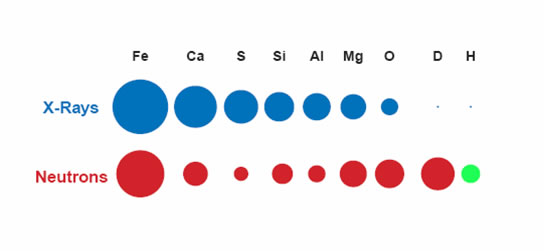
\includegraphics[width=\textwidth]{figures/xrne.png}
  \caption{Comparativa de los tamaños relativos de los spots de difracción
    atómica de neutrones y rayos X.}
  \label{fig:xrne}
\end{figure}

\subsubsection{Extinciones sistemáticas}
El sumatorio en j de las ecuaciones para los factores de forma tiene
implicaciones en el número de \emph{spots} de difracción creados.
\begin{itemize}
\item En estructuras SC, con un solo átomo, el sumatorio solo tiene un miembro,
  y este nunca es nulo.
\item Para dos átomos (estructura FCC) hay ciertas condiciones en que se pueden
  anular los \emph{spots} de difracción.
\item Conforme la estructura posee más átomos por celda, el sumatorio tiene más
  términos y por tanto es más fácil que se den condiciones para que los términos
  sumen cero.
\end{itemize}

\section{Determinación de estructuras}
La dirección de incidencia suele venir fijada por el tubo de rayos X (la óptica
de estas $\lambda$ es muy cara).

El acercamiento más \emph{naive} al problema es incidir y escanear todo el
espacio. Lo estrecho de los picos de difracción ($\sim 0.01^ \circ$) hace de ésta una opción inviable. Por ello, existen geometrías
experimentales que solucionan este problema de maneras distintas, en todos casos
aumentando la cantidad de área en la pantalla que es iluminada por efectos difractivos.

\subsection{Geometría de Laue}
Cogemos un solo cristal. Incidimos con el con radiación ``blanca''
(policromátrica, $\lambda \in (\lambda_i,\lambda_f)$. Esto crea un rontinuo de
esferas de Ewald (fig. \ref{fig:ewaldcontinuum}), y todos los puntos dentro de
este continuo difractan.
\begin{figure}
  \centering
  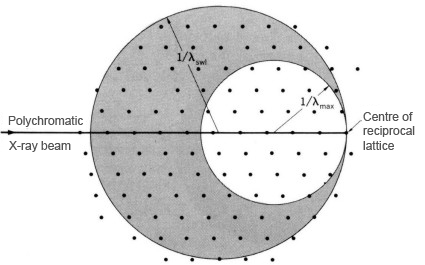
\includegraphics[width=\textwidth]{figures/ewaldcontinuum.png}
  \caption{Todos los puntos contenidos en el continuo de esferas de Ewald
    difractan en la geometría de Laue.}
  \label{fig:ewaldcontinuum}
\end{figure}
La radiación de rayos X tiene una parte ``blanca'' (bremsstrahlung) y otra monocromática (picos), se utiliza la primera parte. El cono de
radiación producido se puede cortar por el detector detrás (reflexión) o delante
(transmisión), como muestra la figura \ref{fig:lauegeom}.
\begin{figure}
  \centering
  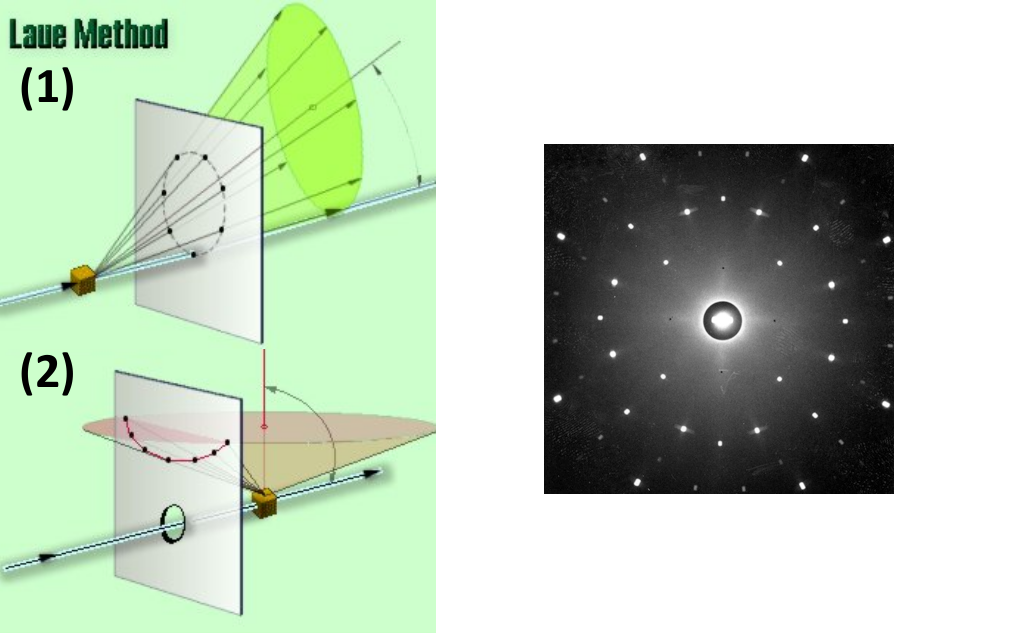
\includegraphics[width=\textwidth]{figures/lauegeom.png}
  \caption{Geometrías posibles para el método de Laue; por reflexión y por
    transmisión. Se muestra también un ejemplo de patrón de difracción típico
    obtenido por este método.}
  \label{fig:lauegeom}
\end{figure}

De la imagen creada, saco los $\mathbf{G}$ y con ellos la red real. Este método
aún se usa para orientar y cortar cristales. 

\subsection{Método del cristal giratorio}
En este caso se utiliza una $\lambda$ única, y se rota el cristal en un eje.
Junto al cristal, rota también la esfera de Ewald (fig. \ref{fig:rotaewald}). La
geometría se muestra en la figura \ref{fig:rotageom}, junto a un ejemplo de
patrón obtenido.

\begin{figure}
  \centering
  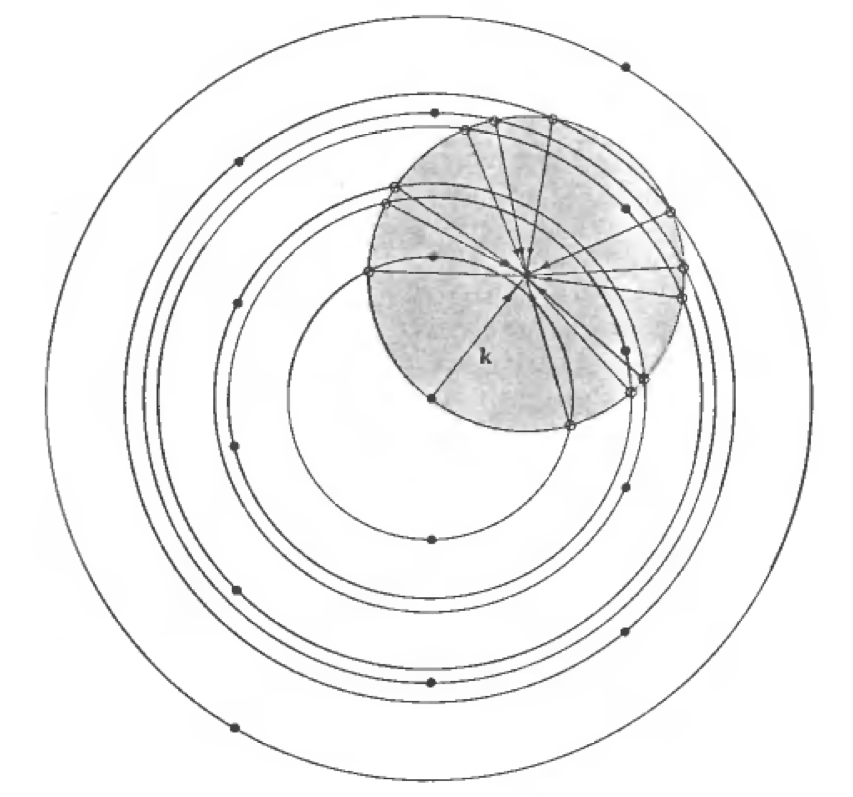
\includegraphics[width=\textwidth]{figures/rotaewald.png}
  \caption{Las esferas de Ewald resultantes en el método del cristal giratorio
    surgen de rotar la inicial. Al rotar el cristal, los planos de éste van
    recorriendo los distintos ángulos de incidencia posibles con la radiación
    incidente, y cuando se cumple la condición de Bragg aparece un spot de
    difracción en la pantalla.}
  \label{fig:rotaewald}
\end{figure}

\begin{figure}
  \centering
  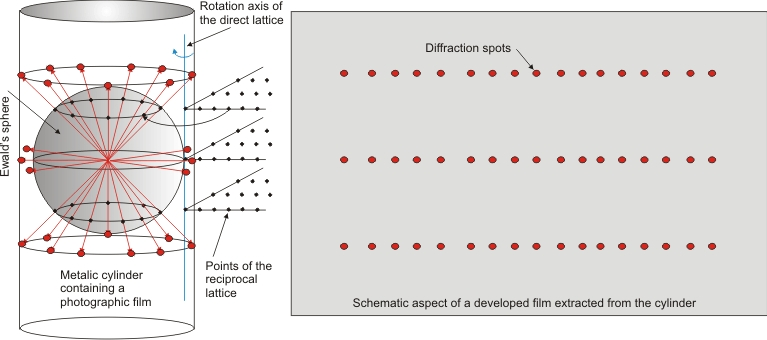
\includegraphics[width=\textwidth]{figures/rotageom.png}
  \caption{Geometría del método del cristal giratorio. La imagen se proyecta en
    un cilindro alrededor de la muestra.}
  \label{fig:rotageom}
\end{figure}



\subsection{Método del polvo (Debye-Scherrer)}
Si no tengo un cristal suficientemente grande, utilizo un polvo de
microcristales (sus tamaños son cercanos a las cinco micras). Tengo una esfera
de Ewald por cristal, por lo que obtengo un cono en lugar de un \emph{spot} de
difracción.

Los cristales están orientados en todas las direcciones del espacio posibles,
así que veo un anillo por cada vez que se cumple la condición de Bragg con ese
plano del cristal en concreto (el anillo viene por la simetría cilíndrica del
problema respecto al rayo incidente). 

El resultado en la pantalla son anillos concéntricos.

\section{Cristales finitos y efectos térmicos}
Si bien la suma de red $\sum_\mathbf{R}e ^{i\mathbf{k}\mathbf{R}}$ debería
diverger, no lo hace por haber un número acotado de $\mathbf{R}$'s.
Para una red 1D, por ejemplo, se tienen $N$ puntos, con separación $a$ en la red
directa y $2\pi/a$ en la recíproca.
\begin{equation}
  \sum_\mathbf{R} e ^{i\mathbf{k}\mathbf{R}} \stackrel{\mathbf{R}=n\mathbf{a}}{=} \sum_{n=0}^{N-1} e ^{ikna} = \Sigma(k)
\end{equation}
Resolvemos multiplicando por $e ^{ika}$ en ambos lados:
\begin{equation}
  \Sigma(k) e ^{ika} = \sum_{n=0}^{N-1} e ^{ika(n+1)} = \Sigma(k)-1+e ^{ikNa}  
\end{equation}
Por tanto
\begin{equation}
    \Sigma(k)=\frac{e ^{ikNa/2}}{e ^{ika/2}} \frac{\sin \frac{kNa}{2}}{\sin \frac{ka}{2}}
\end{equation}
La función intensidad es por tanto (representada en la figura
\ref{fig:comb_finite})
\begin{equation}
  I(\Delta k) \propto \vert \Sigma(\Delta k)\vert^2 = \frac{\sin^2\frac{\Delta k\ Na}{2}}{\sin^2\frac{\Delta k\ a}{2}}
\end{equation}

\begin{itemize}
\item Los máximos principales están distribuidos en las posiciones $\Delta k = m
  \frac{2\pi}{a} = G$, con $m\in \mathbb{N}$. Su valor es $N^2$.
\item Los segundos máximos son un 95\% menos intensos.
\item Para $N$ grande la intensidad tiende a $I(\Delta k) = N^2 \delta_{\Delta k,G}$.
\end{itemize}
En lugar de $k$ se puede utilizar el ángulo $\Delta k = 2k\sin \theta$.

\begin{figure}
  \centering
  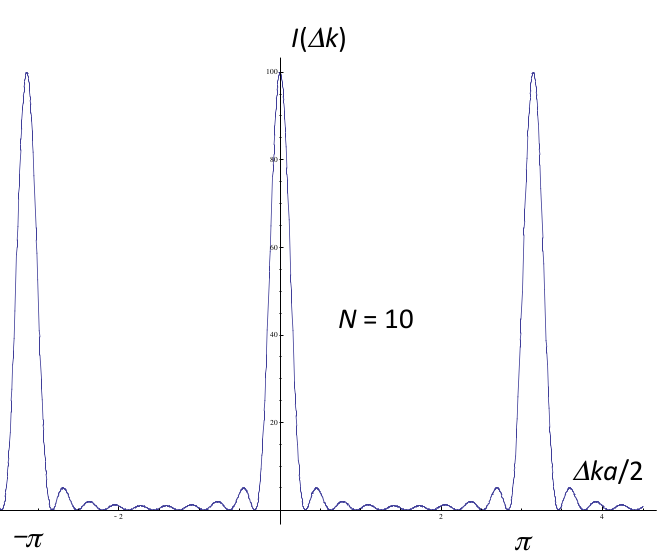
\includegraphics[width=\textwidth]{figures/comb_finite.png}
  \caption{Función intensidad para un cristal de $N=10$.}
  \label{fig:comb_finite}
\end{figure}
\subsection{Fórmula de Scherrer} Si yo asumo que
$\exists \delta(\Delta k)$, relacionando esa anchura con el ángulo vía
$\delta(\Delta k) = 2 \frac{2\pi}{\lambda}\cos \theta \delta \theta$
hallo
$\delta(2\theta) = \frac{\delta(\Delta k)\lambda}{2\pi\cos\theta} =
\frac{\lambda}{\frac{2\pi}{\delta(\Delta k)}\cos \theta} =
\frac{\lambda}{D \cos \theta}$.
En la práctica se suele corregir la fórmula con un factor $k\sim 0.9$.
\begin{equation}
  D \sim \frac{0.9 \lambda}{\delta(2\theta) \cos \theta} \tag{Scherrer's eq.}
\end{equation}
Con $D$ el tamaño de los cristalitos del polvo. La fórmula funciona bien
para $D$ menor de la décima de micra.

\subsection{Efectos térmicos}
Los efectos térmicos se cuantifican con el denotado factor de
\emph{Debye-Waller}. Calculamos el factor de estructura, e incluimos el efecto
de la temperatura perturbando las posiciones ($\mathbf{x}_j \rightarrow
\mathbf{x}_j + \mathbf{u}(T) $):
\begin{equation}
  F(\mathbf{G}) = \sum_j f_j e ^{-i\mathbf{G}\mathbf{x}_j} \sim e ^{-i\mathbf{G}\mathbf{u}} \underbrace{\sum_j f_j e ^{-i\mathbf{G}\mathbf{x}_j}}_{\text{static}}
\end{equation}
Aproximamos los desplazamientos en serie de potencias:
\begin{equation}
\begin{split}
  e ^{-i\mathbf{G}\mathbf{u}} &\sim 1 - i \mathbf{G} \mathbf{u} - \frac{1}{2} (\mathbf{G}\mathbf{u})^2 + \dots \\ 
   \langle e ^{-i\mathbf{G}\mathbf{u}} \rangle &\sim 1 - i \langle \mathbf{G} \mathbf{u} \rangle - \frac{1}{2} \langle (\mathbf{G}\mathbf{u})^2  \rangle+ \dots
\end{split}
\end{equation}
La agitación térmica es estocástica, así que $\mathbf{G}$ y
$\mathbf{u}$ no están correlacionados. Por tanto,
$\langle \mathbf{G}\mathbf{u} \rangle = 0$.

Usando $\mathbf{G}\mathbf{u} = Gu\cos \theta$,
\begin{equation}
  \langle e ^{-i\mathbf{G}\mathbf{u}} \rangle = 1 - \frac{1}{2} G^2
  \langle u^2 \rangle \underbrace{ \langle 
    \cos^2 \theta \rangle}_{\frac{1}{3}} = 
  1 - \frac{1}{6}G^2 \langle u^2 \rangle \simeq e ^{-\frac{1}{6}G\langle u^2 \rangle }
\end{equation}
donde el factor $\nicefrac{1}{3}$ viene de promediar $\cos^2 \theta$
sobre una esfera\footnote{La integral correspondiente es
  $\frac{1}{4\pi} \iint \text{d}\theta\ \sin \theta \ \text{d}\phi\
  [\cos ^2\theta] = \frac{1}{4\pi} 2\pi \cdot \int_0^{\pi} \sin \theta
  \cos ^2\theta \text{d}\theta = \frac{1}{4\pi} 2\pi \cdot
  \nicefrac{2}{3} = \nicefrac{1}{3}$.}.Llegamos, por tanto, a 
\begin{equation}
  I \propto \vert F(G) \vert^2 = I_0 \underbrace{e^{-\frac{1}{3}G^2 \langle u^2 \rangle }
  }_{\mathclap{\text{Debye-Waller factor}}} = I_0 e^{-2 \text{W}}
\end{equation}
Efectos cuánticos hacen que este factor no sea $1$ a $T=0$. En tales
condiciones, conlleva una corrección del 10\%, aproximadamente.

La relación con $T$ del factor se puede estimar con un cálculo
clásico, que es una buena aproximación a altas temperaturas.
\begin{equation}
  \langle U \rangle = \frac{1}{2} M \omega^2 \langle u \rangle ^2 = \frac{3}{2}\kb  T \ \rightarrow \ \langle u \rangle ^2 = \frac{3\kb  T}{M\omega^2}
\end{equation}
Con lo que 
\begin{equation}
  I \sim I_0 e^{-\frac{\kb T}{M\omega^2}G^2}
\end{equation}
La dependencia es muy acusada con G, y por lo tanto con los índices de
Miller.

A bajas temperaturas, recurrimos a los resultados cuánticos para un
oscilador; el sistema está en su estado fundamental y
$\frac{1}{2}M\omega^2 \langle u \rangle ^2 = \frac{3}{4}\hbar \omega$,
por lo que $\langle u \rangle ^2 = \frac{3\hbar}{2M\omega}$ y 
\begin{equation}
  I = I_0 e^{-\frac{\hbar}{2M\omega}G^2} \sim 0.9 I_0
\end{equation}


\chapter{Cohesión en cristales}
En este capítulo, tratamos de responder por qué los cristales son
estructuras favorables energéticamente. Además, vemos por qué
mecanismo se mantiene unido cada cristal (fig \ref{fig:cristalbondings}):
\begin{description}
\item[Metales] Nube electrónica
\item[Cristales iónicos] Interacción electroestática
\item[Cristales covalentes] Estados bonding
\end{description}
\begin{figure}
  \centering
  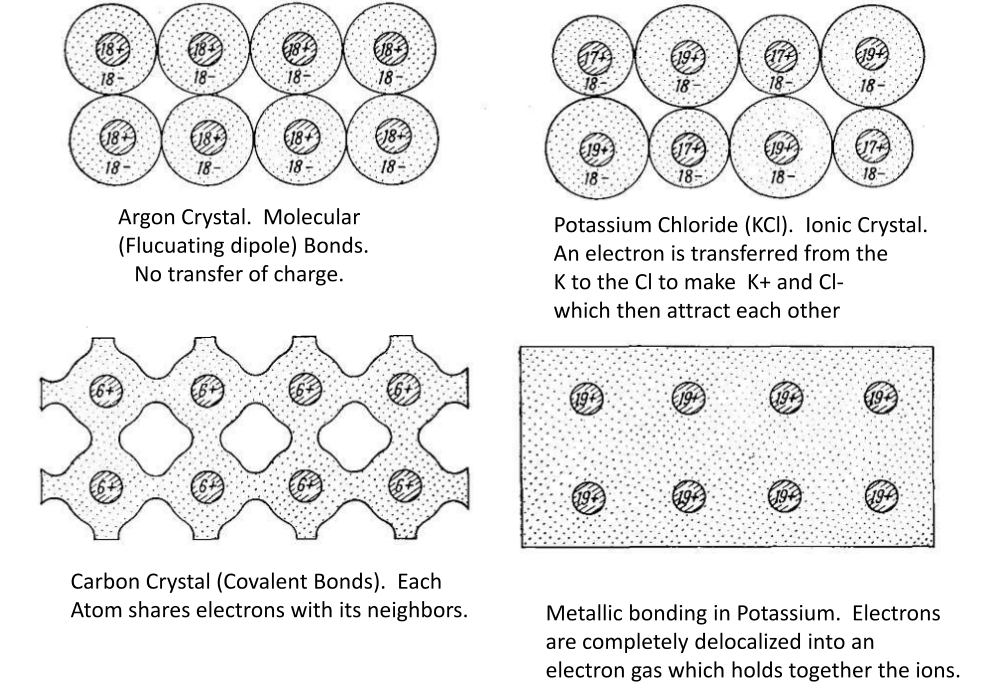
\includegraphics[width=\textwidth]{figures/cristalbondings.png}
  \caption{Mecanismos de unión en cristales.}
  \label{fig:cristalbondings}
\end{figure}

\section{Introducción}
El llenado de orbitales, en primera aproximación parece seguir la
\emph{regla de Madelung}; se llenan de menor a mayor $n+l$. Esta regla
tiene múltiples excepciones, como el cobre ([Ar] 4s\textsuperscript{1} 3d\textsuperscript{10}, no
rellena s\textsuperscript 2) o la plata ([Kr] 5s\textsuperscript 1 4d \textsuperscript{10}, mismo problema).

Diferencias de un sólo electron son importantes, como es el caso del
Ne y el Na. Este electrón de más en el sodio se deslocaliza entre
celdas vecinas (figura \ref{fig:nena}) haciéndolo buen conductor, no
así como el neon sólido.
\begin{figure}
  \centering
  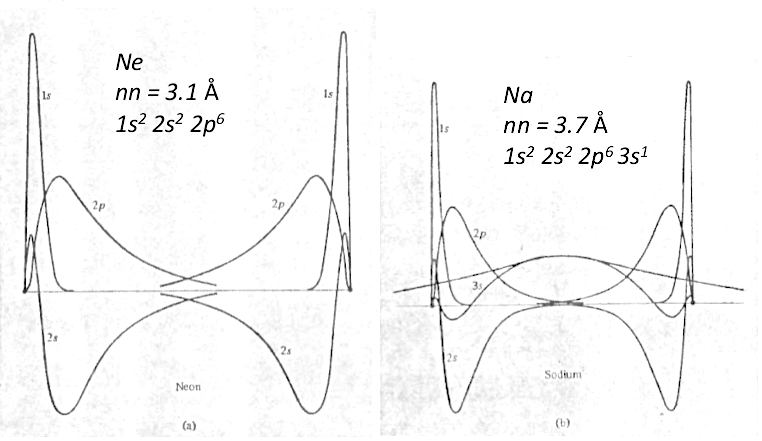
\includegraphics[width=\textwidth]{figures/nena.png}
  \caption{El electrón extra del sodio le da propiedades radicalmente
    diferentes, al establecer un ``puente'' electrónico entre átomos
    en el cristal.}
  \label{fig:nena}
\end{figure}

Definimos el concepto de \emph{energía de cohesión} (por átomo,
molécula, etc.) como
\begin{equation}
  u_0 = \text{Energy of free atoms} - \text{Energy of atoms in cristal
  structure}
\end{equation}
Su valor es de unos 5 eV, y oscila entre valores menores de 0.5 eV
para enlaces de Van der Waals a valores superiores en enlaces iónicos,
metálicos, etc. Los gases nobles tienen energías de cohesión de
aproximadamente 0.1 eV. Es la energía necesaria para ``desensamblar''
el conjunto.

El potencial de interacción es el típico (Lenard-Jones
12-6):
\begin{equation}
  \label{eq:lj126}
  u(r_{12}) = 4\varepsilon \left[ \left(\frac{\sigma}{r_{12}}
    \right)^{12} - \left(\frac{\sigma}{r_{12}} \right)^6 \right]
\tag{LJ 12-6}
\end{equation}

\subsection{Justificación de los exponentes del potencial}
El término repulsivo es el menos importante, siendo sustituible por
cualquier exponencial fuerte (también se usa $\lambda e^{-r/\rho}$,
por ejemplo).  Dediquemos tiempo a justificar el exponente del término
atractivo.


\begin{wrapfigure}{r}{0.5\textwidth}
  \centering
  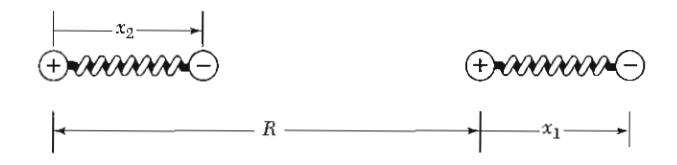
\includegraphics[width=0.48\textwidth]{figures/quantumlj.jpg}
  \caption{Aproximación del átomo.}
  \label{fig:quantumlj}
\end{wrapfigure}

Aproximamos el átomo a dos cargas puntuales unidas por un muelle, de
signo opuesto (fig. \ref{fig:quantumlj}).
Supongamos dos átomos, llamamos a la distancia entre
cargas positivas (los núcleos) $R$, y a las distancias entre las
cargas positivas y negativas de cada átomo $x_1, x_2$. El hamiltoniano
del sistema será la suma de un hamiltoniano básico y otro de
interacción:

\begin{align}
  \mathcal{H}_{\text{basic}} &= \frac{p_1^2}{2m} + \frac{1}{2}C x_1^2
  +\frac{p_2^2}{2m} + \frac{1}{2}C x_2 \tag{Harmonic oscillator}\\
  \mathcal{H}_{\text{int.}} &=
                              \underbrace{\frac{e^2}{R}}_{\text{pos-pos}}
                              + \underbrace{\frac{e^2}{R+x_1-x_2}}_{\text{neg-neg}}
                              +
                              \underbrace{\frac{-e^2}{R+x_1}+\frac{-e^2}{R-x_2}}_{\text{pos-neg}}
                              \tag{Charge interaction}
\end{align}
Suponiendo pequeños desplazamientos para las $x_i$, el hamiltoniano de
interacción se reduce al de dos dipolos:
\begin{equation}
  \mathcal{H}_{\text{int.}} \sim \frac{-2e^2 x_1 x_2}{R^3}
\end{equation}
El hamiltoniano total queda como $  \mathcal{H}= \frac{p_1^2}{2m} + \frac{1}{2}C x_1^2
  +\frac{p_2^2}{2m} + \frac{1}{2}C x_2- \frac{-2e^2 x_1
    x_2}{R^3}$. Notando que es el de una pareja de osciladores
armónicos acoplados, paso a coordenadas normales:
\begin{equation}
  \begin{split}
    x_s &= \frac{1}{\sqrt 2}(x_1 +x_2) \\
    x_a &= \frac{1}{\sqrt 2}(x_1 -x_2) \\
    \mathcal{H}_{\text{N}} &= \frac{p_s^2}{2m} + \frac{1}{2} \left[ C
                             - \frac{2e^2}{R^3} \right] x_s^2 + \\
&+ \frac{p_a^2}{2m} + \frac{1}{2} \left[ C
                             + \frac{2e^2}{R^3} \right] x_a^2 
  \end{split}
\end{equation}
Por tanto, $\omega_{s,a}^2 = \frac{1}{m} \left( C \mp
    \frac{2e^2}{R^3} \right)$. Definiendo $\omega_0$ como $C/m$, y
aproximando $ \frac{2e^2}{CR^3}$ a cero:
  \begin{equation}
    \omega_{s,a} = \omega_0 \left( 1 \mp \frac{2e^2}{CR^3} \right)
    ^{\frac{1}{2}} \sim \omega_0 \left[ 1 \mp \frac{1}{2} \left(
        \frac{2e^2}{CR^3} \right) 
      \pm \frac{1}{8} \left(\frac{2e^2}{CR^3} \  \right)\right]
  \end{equation}
Apliquemos este resultado clásico a dos osciladores cuánticos. A
${T}=0$ se tienen dos osciladores con frecuencias
$\frac{1}{2}\hbar \omega_i$. La diferencia de energías $\Delta u$ si
interaccionan es
\begin{align}
  u_0 &= \frac{1}{2} \hbar \omega_0 + \frac{1}{2} \hbar \omega_0 =  \hbar
  \omega_0 \tag{No int.} \\
  u_0' &= \frac{1}{2} \hbar \omega_s + \frac{1}{2} \hbar \omega_a =  \hbar
         \omega_0 - \frac{1}{8} \hbar \omega_0 \left(
         \frac{2e^2}{CR^3} \right)^2 \tag{Interaction} \\
  \Delta u &= \frac{1}{8} \hbar \omega_0 \left( \frac{2e^2}{CR^3}
               \right)^2 \propto \frac{-1}{R^6}\tag{Interaction effect}
\end{align}

De donde deducimos que la interacción entre átomos esta gobernada por
un exponente de orden seis. Como puede verse, el efecto es puramente cuántico; para
$\hbar \rightarrow 0$ no existe esta interacción.
 
\section{Cristales moleculares}
Son cristales de gases nobles y compuestos orgánicos. Su energía de
cohesión es baja ($\sim 0.1 \text{eV/át.}$), por lo que hay poca
distorsión de la carga. Que las energías de cohesión estén
estrechamente relacionadas con la temperatura de fusión hace que éstas
sean bastante bajas en este tipo de cristales. Su estructura típica es
FCC.

Son aislantes eléctricos (no hay ningún orbital muy solapante entre
átomos que posibilite el transporte de electrones, como en neon en la
figura \ref{fig:nena}) y suelen ser transparentes en el visible.

Tratemos de calcular la energía del cristal. Sumamos a todos los
iones, teniendo en cuenta un potencial tipo Lenard-Jones 12,6 como el
de la ecuación \ref{eq:lj126}:
\begin{equation}
  E_{\text{ion}} = \sum_{j\neq \text{ion}} u(r_{ij})
\end{equation}
Para el cristal, 
\begin{equation}
  E_{\text{cristal}} = N E_{\text{ion}} \cdot \frac{1}{2} =
                       2N\varepsilon \sum_{j \neq i}
                       \left[\left(\frac{\sigma}{r_{ij}}\right)^{12} -
                       \left( \frac{\sigma}{r_{ij}}\right)^6\right] = \dots
\end{equation}
donde se ha utilizado un factor $\frac{1}{2}$ para compensar contar
dos veces a los potenciales de los iones. Simplifiquemos diciendo que
la interacción sólo ocurre a primeros vecinos (la interacción tiene
unos exponentes tan elevados que la corrección es mínima).

Escribiendo $r_{ij} = p_{ij} R$:
\begin{equation}
\begin{split}
  \dots &= 2N\varepsilon \left( \left( \frac{\sigma}{R} \right)^{12}
    \sum_{i\neq j} \left[  \left( \frac{1}{p_{ij}} \right)^{12}
    \right]   - \left( \frac{\sigma}{R} \right)^{6}
    \sum_{i\neq j} \left[  \left( \frac{1}{p_{ij}} \right)^{6}
    \right]\right) =\\ &= 2N\varepsilon \left( \left( \frac{\sigma}{R} \right)^{12}
    S_{12}   - \left( \frac{\sigma}{R} \right)^{6}
S_6  \right)
\end{split}
\end{equation}
donde $S_6$ y $S_{12}$ son dos factores puramente geométricos, que para una
FCC valen $12.13$ y $14.45$.

Con este resultado podemos calcular varios parámetros. Para una FCC:
\begin{description}
\item[Distancia de equilibrio] Es el mínimo del potencial, así que
basta con resolver $\frac{\partial u}{\partial R} = 0$. Se obtiene 
  \begin{equation}
    \frac{R_0}{\sigma}=1.09
  \end{equation}
Las correcciones cuánticas, de valor pequeño (1\%) van como $1/m$.
\item[Energía de cohesión] Se calcula como
  \begin{equation}
    E_{\text{cohesion}} = \frac{E(R_0)}{N} =
    \frac{-S_6^2}{S_{12}}\varepsilon \sim -8.6 \varepsilon
  \end{equation}
El ajuste con los datos experimentales es genial.
\item[Módulo de compresibilidad] El ajuste no es tan bueno como el de
  los demás parámetros.
  \begin{equation}
    B_0 = -V \left( \frac{\partial P}{\partial V} \right) _T =
    \frac{4\varepsilon}{\sigma^3}\frac{S_6^\frac{5}{2}}{S_{12}^
      \frac{3}{2}} \sim 75 \frac{\varepsilon}{\sigma^3}
  \end{equation}
\end{description}

\section{Cristales iónicos}
El ejemplo típico es el cloruro sódico. El Na ha perdido completamente
un e\textsuperscript{-} y el Cl lo ha ganado. El enlace tiene una
fuerza del orden de los 5 eV. 

Nos preguntamos por qué tienen tendencia a cristalizar, y si el enlace
iónico es energéticamente favorable, a pesar de necesitar ionizar los
átomos.

Las energías liberadas y absorbidas al ionizar los átomos del cristal
son, para el NaCl,
\begin{equation*}
  \text{Na} + \SI{5.14}{\eV}\rightarrow \text{Na}^+ + e^-
\end{equation*}
\begin{equation*}
  \text{Cl} + e^- \rightarrow \text{Cl}^- + \SI{3.61}{\eV} 
\end{equation*}
Por lo que hay que aportar \SI{1.53}{\eV} netos por par para ionizar los
átomos. 

En el cristal, la energía entre átomos es deducible suponiendo un
potencial de tipo Lenard-Jones:
\begin{equation}
  u_0 \sim \frac{-1}{4\pi\epsilon_0}\frac{e^2}{R\sim 3 \AA} \sim \SI{-5.12}{\eV} 
\end{equation}
muy cercano al experimental,  \SI{-7.9}{\eV}.

La diferencia de energías al pasar al estado cristalino es, por tanto,
$-5.12 - (-1.53) = -3.59 \text{eV}$, y el estado cristalino es
favorable energéticamente.

\subsection{Energía de Madelung}
La principal contribución a la energía del cristal es la interacción
coulombiana, siendo la interacción de Van der Waals despreciable (un
2\% del total). Se le denota \emph{energía de Madelung}.

\begin{equation}
  u_i = \underbrace{\sum_{i\neq j} \frac{-1}{4\pi \epsilon_0} \frac{\pm
      e^2}{p_{ij}R}}_{\text{Coulomb}} + \underbrace{\sum_{i\neq j}
    \lambda e^{-r_{ij}/\rho}}_{\text{repulsion}}
\end{equation}
donde el $\pm$ tiene un signo u otro dependiendo de si $i,j$ son dos
cargas del mismo signo o del contrario. Viendo que la repulsión a
segundos vecinos es despreciable, y denotando al número de vecinos más
próximos $z$, 
\begin{equation}
  u_i  = \frac{-1}{4\pi \epsilon_0}\frac{e^2}{R}  \underbrace{\left[
  \sum_{i\neq j} \frac{\pm 1}{p_{ij}}\right]}_{\alpha} 
  + \lambda z e^{-R/\rho } 
\end{equation}
Con $\alpha$ la constante de Madelung, púramente geométrica. Su valor
en un cristal FCC es 1.748.

Para $N$ iones, $U = N(-\alpha \frac{e^2}{4\pi \epsilon_0 R} + z
\lambda e ^{-R/\rho})$, de donde podemos calcular $R_0$,
$U_{\text{min}}$ y $B_0$:
\begin{align}
  R_0  &\leftarrow \frac{z\lambda}{\rho} = \frac{\alpha e^2}{4\pi
  \epsilon_0 R^2} \\
  U_0 &= \frac{U(R_0)}{N} = - \frac{\alpha e^2}{4\pi \epsilon_0 R_0}
        \left( 1- \frac{rho}{r_0} \right) \\
\end{align}

\section{Cristales covalentes}
Son cristales formados por compuestos de electronegatividades
similares. Ejemplos son el silicio y los compuestos orgánicos. Las
altas energías de cohesión que poseen (el diamante, por ejemplo, 7.3
eV por átomo) les otorgan altas temperaturas de fusión.

Suelen ser aislantes eléctricos o semiconductores.

Lo que ahora une a los átomos es un estado bonding. Veamos un ejemplo
con un \emph{toy model} del hidrógeno.

\subsection{H\textsubscript{2} toy model}
A $T=0$ estamos en el estado fundamental. Imaginamos el átomo de
H\textsubscript{2} como un pozo cuadrado de potencial, de lado
$L$. Dos átomos de hidrógeno serán equivalentes a dos cajas de lado
$L$, con una onda estacionaria dentro de $\lambda = 2L$ (el estado
fundamental). Cada electron tiene su caja, su espín y una energía de
valor
\begin{equation}
  E = \frac{\pi^2 \hbar^2}{2mL^2}
\end{equation}

Supongamos que esas cajas se aproximan más y más, hasta compartir sus
electrones. Se crea una nueva caja de lado $2L$, en la cual los
electrones están ambos en el estado fundamental (pueden si tienen
distinto spin). La energía de este nuevo estado es:
\begin{equation}
  E' = \frac{\pi^2 \hbar^2}{2m(2L^2)}
\end{equation}
Como $E' < 2E$ el nuevo estado bonding es favorable, como confirman
modelos más complejos.

\section{Enlace metálico}
Este enlace posee una alta energía de cohesión (y temperatura de
fusión), pero no tanto como el covalente. 

Mediante un cálculo semiclásico podemos estimar la energía del sólido.
Suponemos que el cristal es un conjunto de cargas puntuales (los
núcleos) separadas por una distancia $R$ (se supone una estructura HCP
para que sean iguales todas las distancias). Los iones puntuales, de
carga $Q=Ze$, estan rodeados de nubes esféricas de carga $-Ze$ y radio
$R$. La densidad electrónica de esas nubes de carga es $n =
\frac{Ze}{\frac{4}{3}\pi R^3}$, y por tanto, contando el núcleo, la
carga en función del radio es
\begin{equation}
  q(r) = +Ze - n \frac{4}{3}\pi r^3 = Ze \left[ 1 - \left( \frac{r}{R} \right) \right]
\end{equation}
El potencial es, por tanto, $\phi(r) = \frac{q(r)}{4\pi \epsilon_0
  r}$. Siendo $\text{d}E_p = \phi \text{d}q$, se tiene
\begin{equation}
  E_p = \myiiint_0^R \text{d}E_p = \frac{-9z^2 e^2}{40 \pi \epsilon_0 R}
\end{equation}
Con lo que obtenemos la energía potencial por átomo. La energía
cinética es la de un gas de Fermi ($T\sim 0$), bajo el modelo de nube de electrones:
\begin{equation}
  E_c = \frac{3\hbar^2}{10m}\left( 3\pi^2 \frac{N}{V} \right)^{2/3} =
  \frac{3\hbar^2 (9\pi \frac{Z}{4})^{2/3}}{10mR^2}
\end{equation}
La energía total es la suma de la energía potencial y cinética.

Con estos resultados se obtiene la distancia interatómica, $2R_0 =
\frac{4.9 a_0}{Z^{4/3}} \stackrel{z=1}{\sim}2.6 \AA$, y la energía en
$R_0$ (unos \SI{5}{\eV} por átomo). 

El modelo expuesto es incapaz de predecir la estructura del cristal
(FCC, BCC ...), y modelos más útiles son muy complicados, al tratarse
de un problema de muchos cuerpos y cuánticos.
%%% Local Variables:
%%% mode: latex
%%% TeX-master: "../fesi"
%%% End:
